\textbf{Ejemplo 2}\\
Un inversionista tiene dos opciones para invertir su dinero: en la primera opción, puede invertir   COP  200.000 que le retornará   COP  90.000 al final de cada año por los próximos 4 años, en la segunda opción, puede invertir hoy   COP  300.000 y recibir   COP  650.000 al final de 4 años. Si la tasa de interés es del 15\% nominal anual año vencido determinar la mejor alternativa.
\\

\textbf{Solución.}\\
%La tabla ira centrada
\begin{center}
	\renewcommand{\arraystretch}{1.5}% Margenes de las celdas
	%Creación de la cuadricula de 3 columnas
\begin{longtable}[H]{|c|c|c|}
		%Creamos una linea horizontal
\hline
		%Definimos el color de la primera fila
\rowcolor[HTML]{FFB183}
		%%%%% INICIO ASIGNACIÓN PERÍODO FOCAL %%%%%%%
  %%%%%%%%%% INICIO TITULO
  %Lo que se hace aquí es mezclar las 3 columnas en una sola
  \multicolumn{3}{|c|}{\cellcolor[HTML]{FFB183}\textbf{1. Asignación período focal}}   \\ \hline
  %%%%%%%%%% FIN TITULO
  %%%%% INICIO DECLARACIÓN DE VARIABLES %%%%%%%
  \multicolumn{3}{|c|}{$pf = 0 pav$}   \\ \hline
  
%%%%%%%%%%% INICIO TITULO
\rowcolor[HTML]{FFB183}
\multicolumn{3}{|c|}{\cellcolor[HTML]{FFB183}\textbf{2. Declaración de variables}}    \\ \hline
%%%%%%%%%%% FIN TITULO
%%%%%%%%%%% INICIO MATEMÁTICAS

$\quad \quad \quad \quad \quad  R_{1} =   COP  90.000 \quad \quad \quad \quad \quad  $                                     & \multicolumn{2}{c|}{$ VPN=COP ? $} \\
$ R_{2} =   COP  650.000 $	& \multicolumn{2}{c|}{$ VP=COP ?  $} \\
$ i_{1}=15\% naav $	&	\multicolumn{2}{c|}{  } \\

\hline
%%%%%%%%%% FIN MATEMÁTICAS
		%%%%% INICIO FLUJO DE CAJA
\rowcolor[HTML]{FFB183}
\multicolumn{3}{|c|}{\cellcolor[HTML]{FFB183}\textbf{3. Diagrama de flujo de caja}} \\ \hline
		%Mezclamos 3 columnas y pondremos el dibujo
		%%%%%%%%%%%%% INSERCIÓN DE LA IMAGEN
		%Deberán descargar las imágenes respectivas del drive y pegarlas en la carpeta
		%n_capitulo/img/ejemplos/1/capitulo1ejemplo1.pdf  (el /1/ es el numero del ejemplo)
\multicolumn{3}{|c|}{ 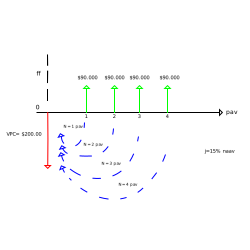
\includegraphics[height=6cm]{E12_3.pdf}} 
   \\ 
\multicolumn{3}{|c|}{ 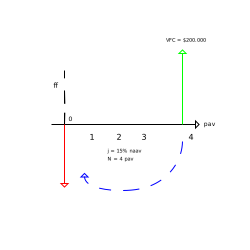
\includegraphics[height=6cm]{E12_4.pdf}} 

   \\\hline
		%%%%%%%%%%%%% FIN INSERCIÓN DE IMAGEN
		%%%%%FIN FLUJO DE CAJA
		
		
		
		%%%%% INICIO DECLARACIÓN FORMULAS
		%%%%%%%%%%% INICIO TITULO
\rowcolor[HTML]{FFB183}
\multicolumn{3}{|c|}{\cellcolor[HTML]{FFB183}\textbf{4. Declaración de fórmulas}}    \\ \hline
%%%%%%%%%%% FIN TITULO
%%%%%%%%%%% INICIO MATEMÁTICAS
\multicolumn{3}{|c|} {$ \quad \quad \quad \quad \quad \quad \quad VPN = \Sigma(Costos) - \Sigma(Inversiones) $\hspace{15pt}\textit{Valor Presente Neto \quad \quad \quad \quad \quad \quad \quad}}   \\ 
\multicolumn{3}{|c|} {$VP = \frac{R}{i}$\hspace{15pt}\textit{ Valor Presente para una Serie Perpetua Vencida}}   \\ 
\multicolumn{3}{|c|} {$B/C = \frac{VPN}{VPC}$\hspace{15pt}\textit{ Relación Beneficio/Costo}}   \\ 
\hline	
	
		%%%%%%%%%% FIN MATEMÁTICAS
		%%%%%% INICIO DESARROLLO MATEMÁTICO
\rowcolor[HTML]{FFB183}
		%%%%%%%%%%INICIO TITULO
\multicolumn{3}{|c|}{\cellcolor[HTML]{FFB183}\textbf{5. Desarrollo matemático}}       \\ \hline
		%%%%%%%%%% FIN TITULO
		%%%%%%%%%% INICIO MATEMÁTICAS
		\multicolumn{3}{|c|}{$ B/C_1 = \frac{  COP  90.000((1+0.15)^{-1}(1+0.15)^{-2}(1+0.15)^{-3}(1+0.15)^{-4})}{  COP  200.000} = 1.28 $}  
		\\
		
		\multicolumn{3}{|c|}{$ B/C_2 = \frac{  COP  650.0000((1+0.15)^{-4})15}{  COP  300.000} = 1.24 $}  
		\\
		\multicolumn{3}{|c|}{$ VPN_1 = -COP 200.000 + COP 90.000((1+0.15)^{-1} $}  
		\\
        \multicolumn{3}{|c|}{$ (1+0.15)^{-2}(1+0.15)^{-3}(1+0.15)^{-4}) = COP 56.948 $}  
		\\
		\multicolumn{3}{|c|}{$ VPN_2 = -COP 300.000 + COP 650.000((1+0.15)^{-4}) = COP 71.540 $}  
		\\
		\multicolumn{3}{|c|}{$ B/C = \frac{COP 540.000(1+0.15)^{-4}}{COP 100.000+COP 90.000((1+0.15)^{-1}(1+0.15)^{-2}(1+0.15)^{-3})}  $}  
		\\
		\multicolumn{3}{|c|}{$ B/C = 1.048 > 0 $}  
		\\
	    \hline
				
		%%%%%%%%%% FIN MATEMÁTICAS
		%%%%%% FIN DESARROLLO MATEMÁTICO
		%%%%%% INICIO RESPUESTA
\rowcolor[HTML]{FFB183}
		%%%%%%%%%%INICIO TITULO
\multicolumn{3}{|c|}{\cellcolor[HTML]{FFB183}\textbf{6. Respuesta}}   \\ \hline
		%%%%%%%%%% FIN TITULO
		%%%%%%%%%% INICIO RESPUESTA MATEMÁTICA
		
\multicolumn{3}{|c|}{ \text{Es mejor elegir la primera opción ya} } \\ 
\multicolumn{3}{|c|}{ \text{que en esta se puede aceptar el exceso de inversión} } \\ 
\hline
		
		
		%%%%%%%%%% FIN MATEMÁTICAS
		%%%%%% FIN RESPUESTA
	\end{longtable}
	%Se crean dos lineas en blanco para que no quede el siguiente texto tan pegado
	%\newline \newline %USARLO SI CREES QUE ES NECESARIO
\end{center}
%%%%%%%%%%%%%%%%%%%%%%%%%%FIN EJERCICIO 1 %%%%%%%%%%%%%%%%%%%%%%%%%%%
